\documentclass[12pt,letterpaper]{article}

\usepackage[hmargin=1in,bottom=1in,top=1in]{geometry}
\usepackage[latin1]{inputenc}
\usepackage{amsmath}
\usepackage{amsfonts}
\usepackage{amssymb}
\usepackage{graphicx}
\usepackage{url}
\usepackage[toc,page]{appendix}
\usepackage{setspace}
\usepackage{pdfpages}
\usepackage{mdwlist}

\usepackage{ulem}
\normalem

% push footnotes to the bottom of the page unconditionally
\usepackage[bottom]{footmisc}

\bibliographystyle{IEEEtran}

\setlength{\parindent}{0in}
\setlength{\parskip}{1.0 \baselineskip}
\setlength{\footnotesep}{1.0 \baselineskip}
\setlength{\skip\footins}{2.0 \baselineskip}

\newenvironment{enumeration}{
	\setlength{\topsep}{0.0pt}
	\setlength{\partopsep}{0pt}
	\setlength{\parskip}{0pt}
	\setlength{\parsep}{0pt}
	\begin{enumerate}
		\setlength{\itemsep}{0pt}}
	{\end{enumerate}}

\newenvironment{itemlist}{
	\setlength{\topsep}{0pt}
	\setlength{\partopsep}{0pt}
	\setlength{\parskip}{0pt}
	\setlength{\parsep}{0pt}
	\begin{itemize}
		\setlength{\itemsep}{0pt}}
	{\end{itemize}}

\newcommand{\sectref}[1]{Section \ref{#1}}
\newcommand{\figref}[1]{Figure \ref{#1}}
\newcommand{\tableref}[1]{Table \ref{#1}}

\begin{document}

\begin{titlepage}
\begin{center}


\includegraphics[scale=1.0]{ecelogo.png}

\vspace{1 \baselineskip}

\textsc{
\Large University of Toronto\\
\large Department of Electrical and Computer Engineering \\
\large ECE496 Design Project
}

\vspace{2 \baselineskip}

{\Large \bfseries Virtual FPGA fabrics} \\
{\Large \bfseries Implementation of a Virtual FPGA Architecture}

\vspace{2 \baselineskip}

{\large \bfseries Individual Progress Report} \\
%{\large \bfseries Final Version}

\vspace{2 \baselineskip}

{\large January 17, 2012}

\vfill

\begin{tabular*}{4in}{l @{\extracolsep{\fill}} l}
\textbf{Neil Isaac} & \texttt{n.isaac@utoronto.ca} \\ & \\
\emph{Project ID:} & 2011017 \\
\emph{Supervisor:} & Jason Anderson \\
\emph{Administrator:} & Ross Gillett \\
\emph{Section:} & \#7 \\
\end{tabular*}

\end{center}
\end{titlepage}

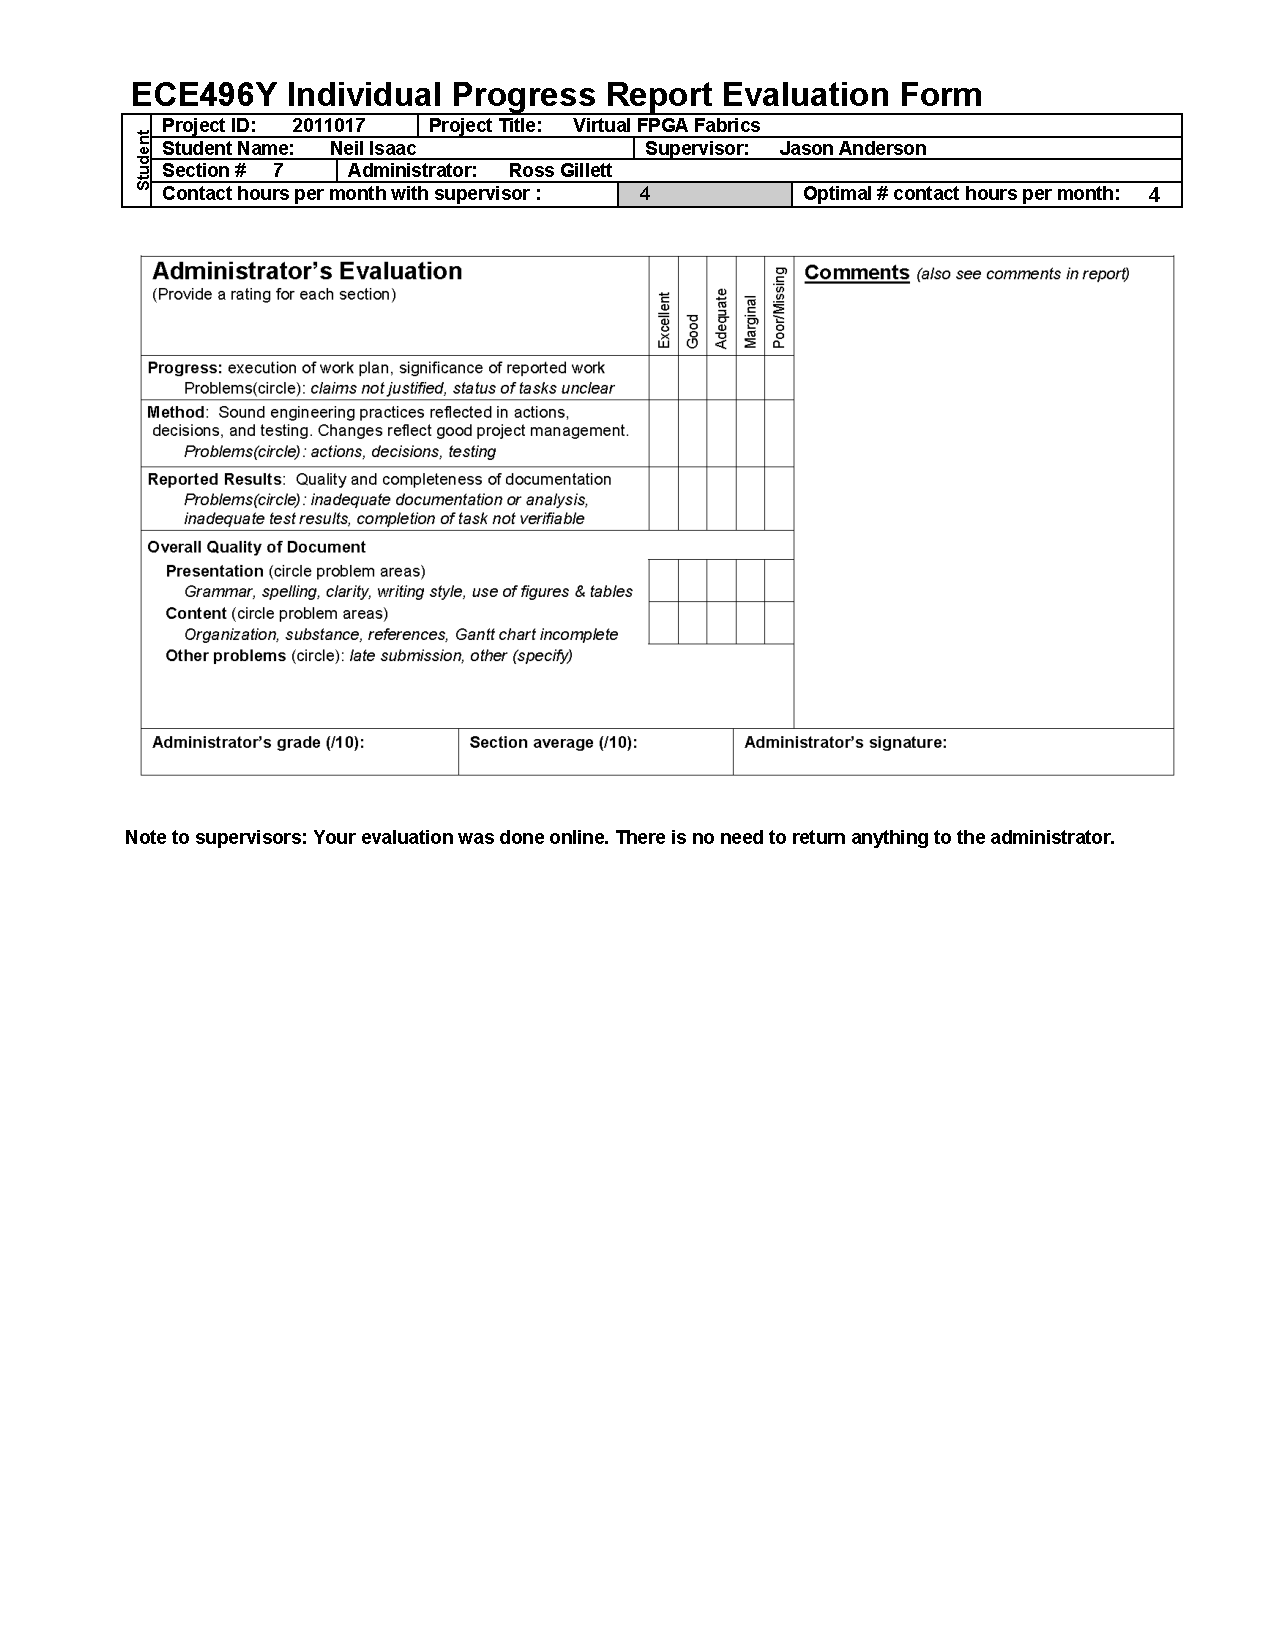
\includepdf{cover-sheet-neil.pdf}

\onehalfspace

\thispagestyle{empty}
\section*{Executive Summary}

blah blah blah


\pagebreak
\pagenumbering{arabic}




\section{Individual Progress and Contributions}

This section lists the major tasks I have been responsible for.
The respective tasks are discussed fully in section 2.

\begin{tabular}{|l|l|l|l|l|l|l|}
\hline
\textbf{Task title} & \textbf{Category} & \textbf{Status} & \textbf{Original date} & \textbf{New date} \\ \hline
\hline
1. Virtual FPGA Verilog code & hardware & completed & Aug-Dec 15 & Aug-Jan 15 \\ \hline
2. External tool flow & tools & completed & Dec 1-15 & Dec 1-15 \\ \hline
3. Bitstream generation software & software & completed & Dec 1-15 & Dec 1-Jan 15 \\ \hline
4. Stress-testing and improvement & testing & not started & Dec 15-Apr & Jan 15-Apr \\ \hline
\end{tabular}




\section{Information on Individual Milestones}

\begin{tabular}{|p{6in}|}
\hline
\textbf{1. Virtual FPGA Verilog code} \\
\emph{Category:} hardware \\
\emph{Original date:} August - December 15 \\
\emph{New date:} August - January 15 \\
\hline
\textbf{Responsibility:} Neil, Keyi \\
The components I wrote were the UART, logic block, connection block, and tile grid. \\
% Keyi: logic element, logic block, shift multiplexing, switch block, logic tile, grid boundary, tile optimization
\hline
\textbf{Status:} completed; future improvements are planned \\
\vspace{-2em}
\begin{itemize*}
\item Verilog code for basic virtual FPGA is complete.
\item Parameters can be changed to create virtual FPGAs of different sizes.
\item Future improvements will aim to to reduce the size of the circuit.
\end{itemize*} 
\vspace{-2em} \\
\hline
\textbf{Actions} \\
\vspace{-2em}
\begin{itemize*}
\item asdf
\end{itemize*} 
\vspace{-2em} \\
\hline
\textbf{Decisions} \\
\vspace{-2em}
\begin{itemize*}
\item asdf
\end{itemize*} 
\vspace{-2em} \\
\hline
\textbf{Testing, verification and results} \\
details \\
\hline
\end{tabular}


\begin{tabular}{|p{6in}|}
\hline
\textbf{2. External tool flow} \\
\emph{Category:} tools \\
\emph{Original date:} December 1 - December 15 \\
\emph{New date:} December 1 - December 15 \\
\hline
\textbf{Responsibility:} Neil \\
\hline
\textbf{Status:} completed \\
details \\
\hline
\textbf{Actions} \\
list \\
\hline
\textbf{Decisions} \\
list \\
\hline
\textbf{Testing, verification and results} \\
details \\
\hline
\end{tabular}


\begin{tabular}{|p{6in}|}
\hline
\textbf{3. Bitstream generation software} \\
\emph{Category:} software \\
\emph{Original date:} December 1- December 15 \\
\emph{New date:} December 1 - January 15 \\
\hline
\textbf{Responsibility:} Neil \\
\hline
\textbf{Status:} completed \\
details \\
\hline
\textbf{Actions} \\
list \\
\hline
\textbf{Decisions} \\
list \\
\hline
\textbf{Testing, verification and results} \\
details \\
\hline
\end{tabular}


\begin{tabular}{|p{6in}|}
\hline
\textbf{4. Stress-testing and improvement} \\
\emph{Category:} testing, hardware \\
\emph{Original date:} December 15 - April \\
\emph{New date:} January 15 - April \\
\hline
\textbf{Responsibility:} Neil, Keyi \\
\hline
\textbf{Status:} completed \\
details \\
\hline
\textbf{Actions} \\
list \\
\hline
\textbf{Decisions} \\
list \\
\hline
\textbf{Testing, verification and results} \\
details \\
\hline
\end{tabular}





\section{Progress Assessment}

blah blah blah




\pagebreak
%\nocite{*} % show uncited entries in the bibliography
\bibliography{ref}
\addcontentsline{toc}{section}{References}

\pagebreak
\begin{appendices}

\section{Gantt Chart}
\label{gantt-chart}

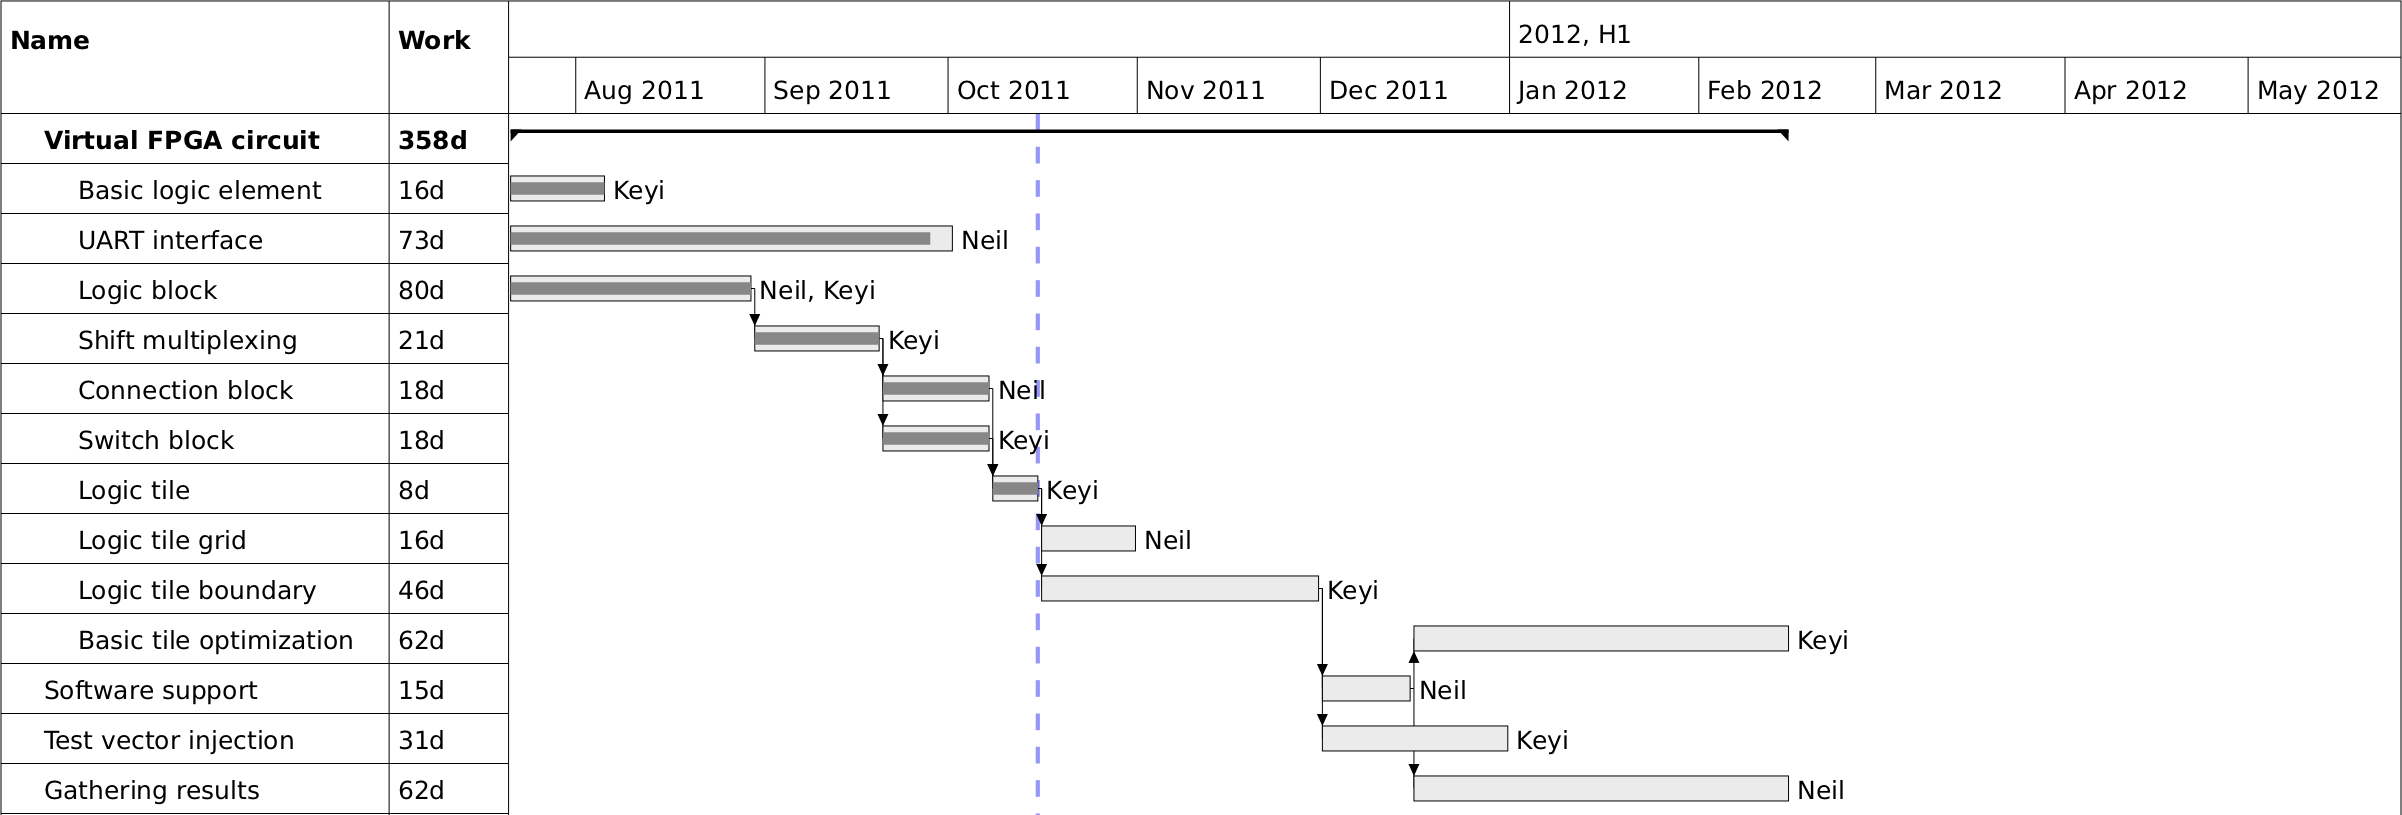
\includegraphics[scale=0.45,angle=90]{gantt.png}



\pagebreak
\section{Test Verilog file}

\begin{verbatim}
module test(
    a, b, c,
    x, y, z,
    clk
);
        
    input a, b, c;
    input clk;
    output x, y, z;

    assign x = a & b;
    assign y = a | b;

    always @ (posedge clk)
        z <= c;

endmodule
\end{verbatim}


\pagebreak
\section{VPR Placement and Routing Result}

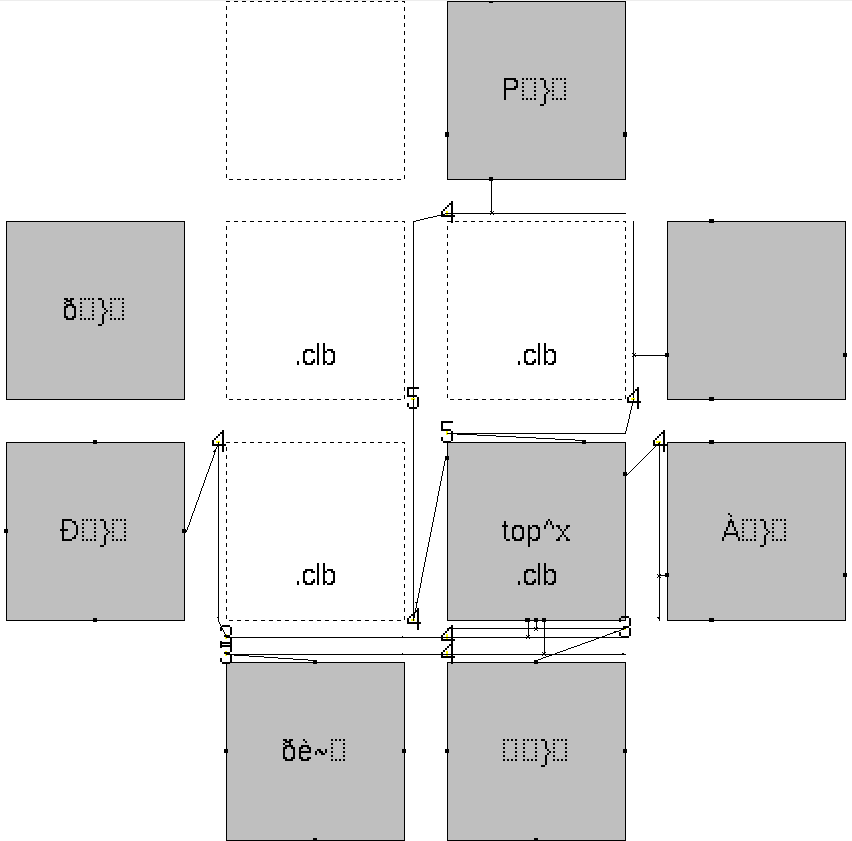
\includegraphics[scale=0.5]{vpr.png}


\end{appendices}

\end{document}


